\documentclass[../../InformazioneQuantistica.tex]{subfiles}

\begin{document}

\chapter{Correlazioni quantistiche}
Nelle precedenti sezioni abbiamo notato come i canali quantistici offrano possibilità in apparenza più ampie dei corrispettivi classici, permettendo per esempio una crittografia sicura o di trasmettere una maggiore \textit{densità} di informazioni. Come sarà chiaro nei prossimi paragrafi, tali opportunità sono consentite dalla presenza di \textit{correlazioni quantistiche non-locali} che non possono essere realizzate da canali puramente classici. Partiremo quindi esaminando i comportamenti non-locali della \MQ (confermati dalla violazione delle disuguaglianze di Bell), per poi cercare metriche per \textit{quantificare} tali correlazioni, mostrando infine che senza di esse risulta del tutto impossibile ottenere risultati simili a quelli esaminati nelle precedenti sezioni. 

\section{Bell Inequalities}
\lesson{10 \orangedot}{28/3/2019}

Nel 1964 John Stewart Bell formulò uno dei più importanti teoremi sui fondamenti della fisica, dimostrando che ogni teoria che si proponga di spiegare determinate misure sperimentali (come la Meccanica Quantistica) debba necessariamente includere comportamenti \textbf{non-locali}. Citando la risposta di Bell stesso in un'intervista del 1988 alla domanda \q{Cosa significa \textbf{località}?}: 
\begin{center} \marginpar{Località}
\q{Si tratta dell'idea che ogni azione abbia conseguenze solo nelle immediate vicinanze, e che ogni conseguenza più lontana sia più debole, e arrivi a destinazione solo dopo un intervallo compatibile con il limite della velocità della luce. La località è l'idea che gli effetti si propaghino \textit{in maniera continua}, che non \textit{saltino} improvvisamente da un punto all'altro.}
\end{center}

\begin{expl}
\textbf{Una definizione rigorosa di località}\cite{Bell-causality}\cite{Stanford-beables}.\index{Località}\\ Una qualsiasi definizione di località è necessariamente ancorata ad una scelta di \q{variabili locali} che si presuppone rispettino la condizione qualitativa appena specificata. Per esempio, il fatto che alla morte della regina di Inghilterra il principe del Galles divenga immediatamente re non risulta in un nessun fenomeno non-locale, dato che una \textit{convenzione} può \q{trasmettersi} a velocità arbitrarie. Analogamente, nella teoria classica dell'elettromagnetismo non sorge alcuna preoccupazione nell'affermare che il potenziale scalare si propaghi con velocità infinita - poiché essendo una grandezza dipendente dalla scelta del \textit{gauge} non è considerata come \q{fisica}, ma solo come un utile ausilio per i conti.\\
Per questo, Bell considera nella sua trattazione della località solo una particolare categoria di \textbf{teorie fisiche}, dette a \q{\textit{beable locali}}.\\
Esplicitamente, una teoria fisica $T$ è un qualsiasi insieme di \textbf{leggi} che consentono di prevedere, a partire da un set di \textbf{informazioni} sul mondo fisico, le \textbf{probabilità} di eventi futuri. Se $X$ è una descrizione completa di un sistema, e $A$ è un possibile evento, la teoria $T$ permette allora di calcolare:
\begin{align*}
X \mapsto P(A|X)
\end{align*}
 Se $T$ è \q{ben specificata}, deve essere chiaro quali siano gli elementi \q{che possono essere considerati reali} (detti \textit{beable})\index{Beable} e che sono oggetto delle leggi, indipendentemente da ogni osservazione. Tali \textit{beable} devono includere, necessariamente, le impostazioni degli apparati sperimentali, e le letture degli strumenti. In altre parole, per poter anche solo introdurre il concetto di località, è necessario che una teoria \textit{assuma} quali grandezze \q{vadano prese seriamente}, ossia abbiano un \q{ruolo privilegiato} rispetto ad eventuali artifizi matematici.\\
Un particolare \textit{beable} è detto \textbf{locale} se corrisponde ad una regione dello spazio fisico (es. il momento di una particella), e \textbf{non-locale} altrimenti (es. la funzione d'onda in MQ, che appartiene ad uno spazio astratto molto più ampio di quello \q{fisico}). Ha senso quindi parlare delle \textit{beable locali} contenute in una regione $R$ dello spaziotempo, mentre \textit{beable non-locali} non sono \q{ancorate} a specifiche posizioni. \\

Consideriamo allora una $T$ che contenga solo \textit{beable locali}, e ci chiediamo se possa essere considerata \textbf{locale} (o \textit{localmente causale}).
Facendo riferimento alla figura \ref{fig:Bell-locality}:
\begin{enumerate}
\item Consideriamo le \textit{beable locali} $b_1$ e $b_2$ (es. setup di apparati ed esiti di misure) contenute rispettivamente nelle regioni $1$ e $2$ separate da un intervallo di tipo spazio.
\item Indichiamo con $3$ una regione, appartenente al passato di $1$, che separi completamente $1$ dal passato di $2$, e contenga tutte le \textit{beable} $B_3$ necessarie affinché la teoria $T$ possa predire le probabilità delle \textit{beable} in $1$.
\item Allora $T$ si dice \textbf{locale} se e solo se specificare le beable in $2$ non modifica le predizioni che si possono già dare per $1$, ossia se:
\begin{align}
\bm{P(b_1|B_3, b_2) = P(b_1|B_3)} \qquad \forall b_2
\label{eqn:prob-locality}
\end{align}
\end{enumerate}
\begin{figure}[H]
\centering
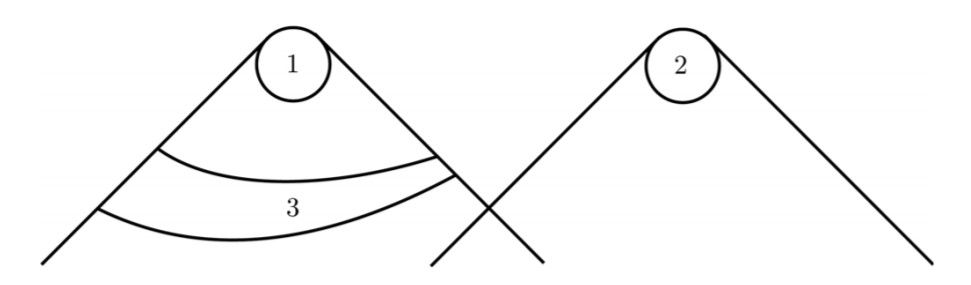
\includegraphics[width=0.7\textwidth]{Immagini/28_3/minkowski1.png}
\caption{In una teoria locale, l'informazione completa contenuta nella regione $3$ del diagramma di Minkowski è sufficiente a determinare le probabilità degli eventi nella regione $1$, indipendentemente da quanto accade nella regione $2$.\label{fig:Bell-locality}}
\end{figure}

Tale definizione permette, grazie al ruolo di $B_3$, di distinguere tra i casi di semplici \textit{correlazioni} e i \textit{sistemi} in cui si ha un effettivo comportamento non-locale.
Per esempio, sia $b_1$ l'evento di \textit{avvenuta cottura di un uovo in una pentola} e $b_2$ lo \textit{squillo di un timer}. Se le informazioni $B_3$ (es. la temperatura dell'acqua, lo stato dell'uovo) consentono di determinare che dopo pochi istanti avverrà $b_1$, il realizzarsi di $b_2$ \q{non modifica la predizione}, e la teoria che consente tali previsioni è locale - nonostante $b_1$ e $b_2$ siano ovviamente fortemente correlati. \\
Se ciò non avviene - per esempio se per qualche motivo l'attivarsi del timer \q{istantaneamente cuoce l'uovo}, dovremmo per forza dedurre che vi è stato un \q{influsso a distanza} del timer sulla cottura dell'uovo. Notiamo che per consentire tale conclusione, $3$ deve rispettare entrambe le ipotesi specificate, ossia essere \textit{completa} e \textit{fungere da barriera}. Se $B_3$ non contiene tutte le informazioni necessarie per predire $b_1$, il realizzarsi di $b_2$ può dare alcune delle informazioni mancanti. Nell'esempio, misurare la temperatura dell'acqua in $B_3$ ma non lo stato dell'uovo non consente di determinare che in $b_1$ sarà cotto, e quindi $b_2$ \q{ha un influsso istantaneo} sulle previsioni - ma questo è dovuto all'ignoranza dello sperimentatore, e non ad un'effettiva non-località.\\
Analogamente, se $B_3$ non scherma $1$ dal passato di $2$, allora possono esservi eventi comuni al passato di $1$ e $2$ che non sono contenuti in $B_3$ e non sono prevedibili dalla sola conoscenza di $B_3$, ma che possono creare correlazioni tra $1$ e $2$, rendendo quindi diverse $P(b_1|B_3,b_2)$ e $P(b_1|B_3)$ (ma solo in teorie stocastiche).\\

Si può estendere il criterio di località anche a teorie $T$ che contengono \textit{beable non-locali}, come la MQ. In questo caso, la condizione (\ref{eqn:prob-locality}) diviene solo necessaria per la località, e le \textit{beable} in $B_3$ comprendono i valori che la funzione d'onda assume su una \q{famiglia di superfici di Cauchy} in $B_3$ (ossia sui luoghi geometrici dello spaziotempo corrispondenti a determinati \q{istanti}).
\end{expl}

Concentriamoci ora sulla definizione matematica di località in un preciso sistema di interesse\cite{Bell-nonlocality}.\\
Consideriamo una sorgente $S$ che produce coppie di qubit entangled (per esempio coppie di particelle con \textit{spin entangled} nell'esperimento di Stern-Gerlach, o fotoni \q{duplicati} da un cristallo non-lineare), che sono fornite a due osservatori, Alice (A) e Bob (B), spazialmente separati (figura \ref{fig:Bell-setup}).\\
Ciascuno dei due ha a disposizione un set di \textit{possibili misure} (permesse dagli apparati di cui è in possesso) che può svolgere sul proprio qubit. Indichiamo con $X$ l'osservabile scelta da Alice, e con $Y$ quella di Bob. A seguito della misura, A otterrà un esito $a \in \sigma(X)$, e B un esito $b\in \sigma(Y)$.
\begin{figure}[H]
\centering
\tikzset{every picture/.style={line width=0.75pt}} %set default line width to 0.75pt        

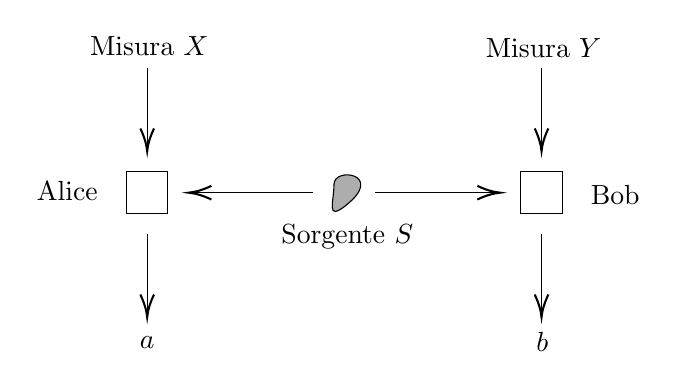
\begin{tikzpicture}[x=0.75pt,y=0.75pt,yscale=-1,xscale=1]
%uncomment if require: \path (0,300); %set diagram left start at 0, and has height of 300

%Shape: Square [id:dp9196862351413921] 
\draw   (260,120) -- (280,120) -- (280,140) -- (260,140) -- cycle ;
%Straight Lines [id:da17930112223236172] 
\draw    (270,70) -- (270,108) ;
\draw [shift={(270,110)}, rotate = 270] [color={rgb, 255:red, 0; green, 0; blue, 0 }  ][line width=0.75]    (10.93,-3.29) .. controls (6.95,-1.4) and (3.31,-0.3) .. (0,0) .. controls (3.31,0.3) and (6.95,1.4) .. (10.93,3.29)   ;

%Straight Lines [id:da47107310700179994] 
\draw    (270,150) -- (270,188) ;
\draw [shift={(270,190)}, rotate = 270] [color={rgb, 255:red, 0; green, 0; blue, 0 }  ][line width=0.75]    (10.93,-3.29) .. controls (6.95,-1.4) and (3.31,-0.3) .. (0,0) .. controls (3.31,0.3) and (6.95,1.4) .. (10.93,3.29)   ;

%Straight Lines [id:da3446633388248408] 
\draw    (350,130) -- (292,130) ;
\draw [shift={(290,130)}, rotate = 360] [color={rgb, 255:red, 0; green, 0; blue, 0 }  ][line width=0.75]    (10.93,-3.29) .. controls (6.95,-1.4) and (3.31,-0.3) .. (0,0) .. controls (3.31,0.3) and (6.95,1.4) .. (10.93,3.29)   ;

%Straight Lines [id:da822622270040033] 
\draw    (380,130) -- (438,130) ;
\draw [shift={(440,130)}, rotate = 180] [color={rgb, 255:red, 0; green, 0; blue, 0 }  ][line width=0.75]    (10.93,-3.29) .. controls (6.95,-1.4) and (3.31,-0.3) .. (0,0) .. controls (3.31,0.3) and (6.95,1.4) .. (10.93,3.29)   ;

%Shape: Square [id:dp7370593336819211] 
\draw   (450,120) -- (470,120) -- (470,140) -- (450,140) -- cycle ;
%Straight Lines [id:da5563468788997123] 
\draw    (460,70) -- (460,108) ;
\draw [shift={(460,110)}, rotate = 270] [color={rgb, 255:red, 0; green, 0; blue, 0 }  ][line width=0.75]    (10.93,-3.29) .. controls (6.95,-1.4) and (3.31,-0.3) .. (0,0) .. controls (3.31,0.3) and (6.95,1.4) .. (10.93,3.29)   ;

%Straight Lines [id:da6249187435301291] 
\draw    (460,150) -- (460,188) ;
\draw [shift={(460,190)}, rotate = 270] [color={rgb, 255:red, 0; green, 0; blue, 0 }  ][line width=0.75]    (10.93,-3.29) .. controls (6.95,-1.4) and (3.31,-0.3) .. (0,0) .. controls (3.31,0.3) and (6.95,1.4) .. (10.93,3.29)   ;

%Curve Lines [id:da7601728877448455] 
\draw [color={rgb, 255:red, 0; green, 0; blue, 0 }  ,draw opacity=1 ][fill={rgb, 255:red, 173; green, 173; blue, 173 }  ,fill opacity=1 ]   (365.5,136.33) .. controls (385,121) and (360,117.33) .. (360,126) .. controls (360,134.67) and (356,143.67) .. (365.5,136.33) -- cycle ;



% Text Node
\draw (231.5,129) node  [align=left] {Alice};
% Text Node
\draw (495.5,131) node  [align=left] {Bob};
% Text Node
\draw (366.4,151) node  [align=left] {Sorgente $\displaystyle S$};
% Text Node
\draw (271,59.5) node  [align=left] {Misura $\displaystyle X$};
% Text Node
\draw (461,60.5) node  [align=left] {Misura $\displaystyle Y$};
% Text Node
\draw (270,202) node   {$a$};
% Text Node
\draw (460.33,201.67) node   {$b$};


\end{tikzpicture}
\caption{Schema dell'esperimento di Bell per esaminare la non-località della \MQ. Una sorgente $S$ di coppie di particelle entangled invia una particella ad Alice e una a Bob, che eseguono rispettivamente una misura $X$ e $Y$ sulla loro particella, ottenendo come risultati $a$ e $b$\label{fig:Bell-setup}}
\end{figure}

In generale, ripetendo l'esperimento (partendo sempre dallo stesso stato iniziale), Alice potrà ottenere un risultato $a'\neq a$, e Bob un $b'\neq b$, a seconda della natura (potenzialmente diversa) delle misurazioni $X$ e $Y$ effettuate, o di incertezze intrinseche al sistema. In ogni caso, abbiamo a disposizione una teoria $T$ che permette di determinare la probabilità $P(a,b|X,Y)$ di ottenere come esiti $a$ e $b$ per una specifica scelta di $X$ e $Y$.

\begin{enumerate}
\item Non è detto che tale probabilità sia fattorizzabile:
\begin{align*}
P(a,b|X,Y) \neq P(a|X)P(b|Y)
\end{align*}
poiché potrebbero essere presenti \textbf{correlazioni} tra esiti di misure diverse (per esempio $b$ potrebbe dipendere dal risultato $a$ di Alice).\\ %Inserire un esempio
 La sola presenza di correlazioni, tuttavia, non significa che vi siano fenomeni non-locali in gioco: le correlazioni potrebbero essere dovute all'origine comune delle particelle misurate.
\item Supponiamo che la teoria $T$ sia \textbf{locale}, e che le misurazioni di A e B avvengano in regioni $1$ e $2$ separate da un intervallo di tipo spazio (figura \ref{fig:Bell-diagram}). 
\begin{figure}[H]
\centering
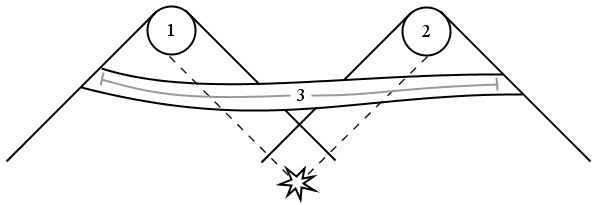
\includegraphics[width=0.7\textwidth]{Immagini/28_3/minkowski2.png}
\caption{Diagramma di Minkowski per lo scenario di Bell. Gli apparati di Alice e Bob si trovano nelle regioni $1$ e $2$, e lo stato del sistema è definito nella regione $3$.\label{fig:Bell-diagram}}
\end{figure}

L'unico modo per spiegare le correlazioni tra $a$ e $b$ è allora dato dall'esistenza di parametri $\lambda$ che \textit{definiscono lo stato iniziale} (nella regione $3$) e che permettano di calcolare le probabilità $P(a,b|X,Y,\lambda)$.
In altre parole, in una teoria locale devono esistere \q{parametri locali} che sono già definiti quando le particelle sono separate, prima della misura, e che ne descrivono completamente il comportamento - spiegando di conseguenza ogni correlazione. 

\item I parametri $\lambda$ possono anche non essere misurabili (\q{variabili nascoste}), ma possiamo osservarne l'effetto nelle correlazioni misurate. Poiché le $\lambda$ contengono già tali correlazioni, la probabilità condizionata diviene ora separabile:
\begin{align}\label{eqn:fattorizzabilita}
P(a, b|X,Y,\lambda) = P(a|X,\lambda)\cdot P(b|Y,\lambda).
\end{align}



\begin{expl}
\textbf{Derivazione della fattorizzabilità.}\index{Località!Fattorizzabilità}
Le osservabili scelte e i loro esiti $a,b,X,Y$ sono infatti \textit{beable} delle regioni $1$ e $2$. Se $T$ è locale, allora possiamo individuare una regione $3$ tali che le \textit{beable} $\lambda$ in esse contenute permettano di calcolare le probabilità degli eventi in $1$ e in $2$, e che separi ciascuna regione dal passato dell'altra. Si ha allora che ogni esito $a,b$ dipende esclusivamente da $\lambda$ e dal relativo setup sperimentale ($X,Y$) che si trova nella stessa regione:
\begin{align*}
P(a|X,Y,b,\lambda) &= P(a|X,\lambda)\\
P(b|X,Y,a,\lambda) &= P(b|Y,\lambda)
\end{align*}
In particolare, notando che anche $P(b|X,Y,\lambda)=P(b|Y,\lambda)$ e che, per la definizione di probabilità condizionata, vale:
\begin{align*}
P(a,b|X,Y,\lambda) = P(a|X,Y,b|\lambda) \cdot P(b|X,Y,\lambda)
\end{align*}
troviamo:
\begin{align*}
P(a,b|X,Y,\lambda)=P(a|X,\lambda) \cdot P(b|Y,\lambda)
\end{align*}
In realtà perché ciò valga è richiesta anche l'ipotesi che la scelta di $X$ e $Y$ non modifichi il valore di $\lambda$ (la cosiddetta \q{free choice} o \q{\textbf{no conspiracy}}). Ciò è sensato, poiché la regione $3$ può contenere un numero enorme di \textit{beable}, e quelle che influenzano $a$ e $b$ possono essere scelte distinte da quelle che influenzano $X$ e $Y$. Così facendo, una diversa scelta di $X$ e $Y$ comporta una variazione della \q{parte di $\lambda$} che non ha alcun effetto su $a$ e $b$, e quindi la fattorizzazione vale ancora.\\
Per esempio, consideriamo un \textit{trial} per un nuovo farmaco, in cui misuriamo l'effetto del farmaco ($X_1$) o di un placebo ($X_2$) su pazienti diversi. L'esito ($a$) del test dipende da delle condizioni $\lambda$ (es. salute del paziente, sensibilità al principio attivo, etc.) che si presume siano completamente diverse da quelle usate per scegliere se somministrare il farmaco o meno (es. lanciare una moneta). Perciò si può dire che $X_1$ e $X_2$ non influenzano \q{la parte di $\lambda$} rilevante per l'esito $a$.\\
Rigettare tale ipotesi significa affermare l'esistenza di una qualche \q{cospirazione} che spinge gli sperimentatori ad assegnare il farmaco solo ai pazienti meno recettivi, cosa che è del tutto irragionevole, e mina i fondamenti stessi della possibilità di condurre esperimenti.\\

\textbf{Nota}: dato che la regione $3$ interseca i passati di entrambe le regioni $1$ e $2$, nella definizione \textit{generalizzata} di località possiamo considerare tra le informazioni contenute in $3$ anche una funzione d'onda \textit{non separabile} (cioè entangled) che descriva lo stato delle due particelle. 
\end{expl}

\item In generale, $\lambda$ può cambiare nel tempo (es. da un esperimento all'altro). Possiamo allora pensare a $\lambda$ come una variabile casuale, che assume valori $\lambda \in \Lambda$ e si distribuisce secondo la densità di probabilità $q(\lambda)$. Sperimentalmente ci interessano allora le probabilità \textit{marginalizzate}, ossia:
\begin{align}
P(a,b|X,Y)=\int_\Lambda d\lambda\,q(\lambda) p(a|X,\lambda) p(b|Y,\lambda)
\label{eqn:prob-cond-final}
\end{align}
\end{enumerate}

L'introduzione di variabili nascoste permette di spiegare (per esempio) come un sistema intrinsecamente deterministico \textit{appaia} indeterministico, non avendo accesso a \textit{tutte} le informazioni che ne descrivono lo stato. Per esempio, potremmo pensare ad un modello come il seguente.\\
Consideriamo come base computazionale $\{\ket{\uparrow}_z, \ket{\downarrow}_z\}$ gli autostati di $\hat{\sigma}_z$ (spin lungo $\hat{z}$ per un fermione). Lo stato $\ket{\psi}$ di un generico qubit è allora dato da:
\begin{align*}
\ket{\psi} = \cos\frac{\theta}{2}\ket{\uparrow} + \sin\frac{\theta}{2} \ket{\downarrow} \qquad \theta \in [0,2\pi)
\end{align*}
Una misura di $\ket{\psi}$ è indeterminata, nel senso che possiamo calcolare a priori solamente la probabilità di un particolare esito. In particolare, si ottiene $\ket{\uparrow}$ con $p=\cos^2 \theta/2$, e $\ket{\downarrow}$ con probabilità $1-p$.\\
Tuttavia, potremmo considerare un modello in cui al qubit è associato un \textit{parametro locale} $\lambda \in[0,1]$, uniformemente distribuito e non misurabile, che codifica l'esito delle future misure: 
\begin{itemize}
\item $\ket{\uparrow}$ se $0 \leq \lambda \leq \cos^2 \frac{\theta}{2}$
\item $\ket{\downarrow}$ se $\cos^2 \frac{\theta}{2} \leq \lambda \leq 1$
\end{itemize}
Poiché non sappiamo $\lambda$, non possiamo determinare a priori il risultato di una misura di spin, ma possiamo solo darne una \textbf{probabilità} - ritroviamo quindi la descrizione data dalla funzione d'onda in \MQ, con il postulato di Bohr sulle probabilità.\\

\textbf{Nota}: il teorema di Bell non riguarda solamente le teorie alle variabili nascoste \textit{deterministiche}, ma offre condizioni che devono essere rispettate da \textit{ogni teoria locale}. In effetti, la condizione di località (\ref{eqn:fattorizzabilita}) è formulata in termini di sole probabilità.

\index{Teorema!Bell}
\begin{thm}
Le predizioni $P(ab|XY)$ date dalla \MQ non ammettono una decomposizione della forma (\ref{eqn:prob-cond-final}). Poiché la (\ref{eqn:prob-cond-final}) è una condizione necessaria perché una teoria sia considerabile locale, ogni teoria compatibile con le predizioni della \MQ (verificate sperimentalmente) è quindi di carattere non-locale.
\end{thm}
\textbf{Dimostrazione}.\\
Consideriamo uno scenario in cui Alice e Bob hanno ciascuno a disposizione due apparati di misurazione, per cui $X \in \{x_0, x_1\}$ e $Y\in \{y_0, y_1\}$. Supponiamo che l'esito di ogni possibile misura sia binario, ossia $a, b \in \{-1,1\}$.\\
Indicheremo con $\langle a_x b_y \rangle$ il valor medio del prodotti degli esiti $a, b$ per una scelta fissata delle misure $(x,y)$. Per esempio, $\langle a_0 b_0\rangle$ è il valor medio di $a \cdot b$ quando $X=x_0$ e $Y=y_0$.\\
Esplicitamente:
\begin{align}
\langle a_x b_y\rangle \equiv \sum_{a,b\in\{-1,1\}} a\,b\,p(a,b|X,Y)
\label{eqn:correlatore}
\end{align}
L'idea è ora quella di considerare un'\textit{arbitraria} funzione $S$ delle correlazioni $\langle a_x b_y \rangle$, che ha la caratteristica di essere quella giusta per dimostrare il teorema:
\begin{align}
S= \langle a_0 b_0 \rangle + \langle a_0 b_1\rangle + \langle a_1 b_0 \rangle - \langle a_1 b_1 \rangle 
\label{eqn:S-Bell}
\end{align}
Dimostriamo ora che in una teoria locale (dove quindi vale la fattorizzazione (\ref{eqn:prob-cond-final})) deve essere $\bm{S\leq 2}$ (\textbf{disuguaglianza CHSH}).\marginpar{Disuguaglianza CHSH}\\
Tuttavia, calcolando $S$ tramite la \MQ, e valutando i valor medi per uno stato massimamente entangled (es. uno stato di Bell), troveremo che $S \leq 2$ non vale: e quindi la (\ref{eqn:prob-cond-final}) non può essere compatibile con le predizioni della \MQ.\\

Partiamo quindi supponendo di essere in una teoria locale, per cui vale la (\ref{eqn:prob-cond-final}). Inserendola in (\ref{eqn:correlatore}) otteniamo:
\begin{align*}
\langle a_x b_y \rangle &\underset{(\ref{eqn:prob-cond-final})}{=} \sum_{a,b\in\{-1,1\}} a\,b \int_\Lambda d\lambda q(\lambda) p(a|X,\lambda) p(b|Y,\lambda) =\\
&=
 \int_\Lambda d\lambda\, q(\lambda) \sum_{a,b \in\{-1,1\}} a\, b\, p(a|X,\lambda)p(b|Y,\lambda)=\\
&= \int_\Lambda d\lambda\, q(\lambda)\underbrace{\left(\sum_{a\in \{-1,1\}} a\, p(a|X,\lambda)\right)}_{\langle a_x \rangle_\lambda} \underbrace{\left(\sum_{b\in \{-1,1\}} b\, p(b|Y,\lambda)\right)}_{\langle b_y \rangle_\lambda} = \int_\Lambda d\lambda\, q(\lambda) \langle a_x\rangle_\lambda \langle b_y\rangle_\lambda
\end{align*}
dove $\langle a_x\rangle_\lambda$ e $\langle b_y\rangle_\lambda$ sono i valori medi degli esiti $a$ e $b$ per una scelta di $(x,y,\lambda)$.\\
Sostituendo tale risultato in (\ref{eqn:S-Bell}) troviamo:
\begin{align*}
S &= \int_\Lambda d\lambda \, q(\lambda) S_\lambda \\
S_\lambda &\equiv \langle a_0 \rangle_\lambda \langle b_0 \rangle_\lambda + \langle a_0\rangle_\lambda \langle b_1 \rangle_\lambda + \langle a_1 \rangle_\lambda \langle b_0 \rangle_\lambda - \langle a_1 \rangle_\lambda \langle b_1 \rangle_\lambda
\end{align*}
Poiché $a$ e $b$ possono assumere valori tra $\{-1,+1\}$, i vari valor medi devono essere compresi tra $-1$ e $1$:
\begin{align*}
\langle a_x \rangle_\lambda \in [-1,1] \qquad \langle b_y\rangle_\lambda \in [-1,1]
\end{align*}
Ma allora si ha:
\begin{align*}
S_\lambda = \langle a_0 \rangle_\lambda \left[ \langle b_0\rangle_\lambda + \langle b_1 \rangle_\lambda \right] + \langle a_1 \rangle_\lambda \left[\langle b_0 \rangle_\lambda - \langle b_1 \rangle_\lambda \right] \leq  |\langle b_0 \rangle_\lambda + \langle b_1 \rangle_\lambda | + |\langle b_0\rangle_\lambda - \langle b_1 \rangle_\lambda|
\end{align*}
dato che è possibile massimizzare $S_\lambda$ scegliendo $\langle a_{0,1}\rangle_\lambda$ in modo che i termini tra parentesi quadre siano entrambi positivi. Precisamente, per la prima parentesi:
\begin{align*}
\langle a_0\rangle(\langle b_0\rangle + \langle b_1\rangle) \leq \max[-1\cdot (\langle b_0\rangle + \langle b_1\rangle); +1\cdot (\langle b_0 \rangle + \langle b_1 \rangle)] = |\langle b_0\rangle + \langle b_1 \rangle ]
\end{align*}
e una relazione analoga si ha anche per la seconda.\\
Siamo allora giunti a:
\begin{align*}
S_\lambda \leq |\langle b_0 \rangle + \langle b_1 \rangle| + |\langle b_0 \rangle - \langle b_1 \rangle|
\end{align*}
Possiamo supporre, senza perdita di generalità, che $\langle b_0 \rangle \geq \langle b_1 \rangle \geq 0$, e quindi rimuovere i due valori assoluti e trovare:
\begin{align*}
S_\lambda \leq 2\langle b_0\rangle \leq 2
\end{align*}

\begin{expl}
Equivalentemente, siano $x,y\in [-1,1]$, allora $S_\lambda=|x+y|+|x-y|\leq 2$. Infatti, prendendo il quadrato:
\begin{align*}
S^2_\lambda = x^2 + y^2 +2xy +x^2+y^2 -2xy + 2|x+y||x-y| = 2x^2 +2y^2 +2|x^2-y^2|
\end{align*}
che è uguale a $4x^2$ o a $4y^2$, e in entrambi i casi è $S^2_\lambda\leq 4\Rightarrow S_\lambda\leq 2$.
\end{expl}
Si ha allora:
\begin{align*}
S = \int_\Lambda d\lambda q(\lambda) S_\lambda \leq 2\int_\Lambda d\lambda q(\lambda) = 2\Rightarrow S\leq 2
\end{align*}
dato che $q(\lambda)$ è normalizzata.\\



Svolgiamo ora lo stesso calcolo\marginpar{Violazione della disuguaglianza CHSH in \MQ} con il formalismo della \MQ. Consideriamo la base computazionale $\{\ket{0},\ket{1}\}$ degli autostati di $\hat{\sigma}_z$. Nella \MQ, l'informazione completa ($\lambda$) necessaria per calcolare le probabilità di ogni misura è contenuta nello stato $\ket{\psi}$ dei due qubit, che supponiamo essere \textit{massimamente entangled}, ossia pari allo stato di singoletto $\ket{\psi^-}$:
\begin{align*}
\ket{\psi^-}=\frac{1}{\sqrt{2}}(\ket{01}-\ket{10})_{AB}
\end{align*}
Supponiamo che Alice e Bob possano misurare lo spin delle rispettive particelle in arbitrarie direzioni $\vec{X}$ e $\vec{Y}$ ($\in \bb{R}^3$). Esplicitamente, ($X,Y$) sono quindi scelte di osservabili del tipo:
\begin{align*}
\hat{O}_x = \vec{X}\cdot \vec{\sigma} \qquad \hat{O}_y = \vec{Y}\cdot \vec{\sigma}; \qquad \vec{\sigma} = (\sigma_x, \sigma_y,\sigma_z)
\end{align*}
Detti $\vec{X} = (X_1, X_2, X_3)^T$ e $\vec{Y}=(Y_1, Y_2, Y_3)^T$, nella base computazionale di un qubit:
\begin{align*}
\vec{X} \cdot \vec{\sigma} = \begin{pmatrix} X_3 & X_1-iX_2\\ X_1 +iX_2 & -X_3\end{pmatrix}; \qquad \vec{Y} \cdot \vec{\sigma} = \begin{pmatrix} Y_3 & Y_1-iY_2\\ Y_1+iY_2 & -Y_3 \end{pmatrix}
\end{align*}
Le singole correlazioni che compaiono in $S_\lambda$ sono quindi date da:
\begin{align*}
\langle a_x b_y\rangle &= \bra{\psi^-}(\vec{X} \cdot \vec{\sigma})_A \otimes (\vec{Y} \cdot \vec{\sigma})_B \ket{\psi^-}
\end{align*}
Nella base computazionale per $2$ qubit $\{\ket{00}, \ket{01}, \ket{10}, \ket{11}\}$ vale:
\begin{align}\label{eqn:corr-mq}
\langle a_xb_y \rangle &= \frac{1}{2} \begin{pmatrix} 0 & 1 & -1 & 0 \end{pmatrix} M \begin{pmatrix} 
0 \\ 1 \\ -1 \\ 0
\end{pmatrix} = - \vec{X}\cdot \vec{Y} \\ \nonumber
M&= 
 \resizebox{0.8\hsize}{!}{%
$\left({\begin{array}{cc|cc}
X_3 Y_3 & X_3(Y_1-iY_2) & (X_1-iX_2)Y_3 & (X_1-iX_2)(Y_1-iY_2)\\
X_3(Y_1+iY_2) & -X_3 Y_3 & (X_1-iX_2)(Y_1+iY_2) & -Y_3(X_1-iX_2)\\ \midrule 
(X_1+iX_2)Y_3 & (X_1+iX_2)(Y_1-iY_2) & -X_3Y_3 &-X_3(Y_1-iY_2)\\
(X_1+iX_2)(Y_1+iY_2) & -Y_3(X_1+iX_2) & -X_3(Y_1+iY_2) & X_3Y_3
\end{array}} \right)$ }
\end{align}
Restringiamoci al caso in cui Alice e Bob possano misurare solo lungo due direzioni \textit{opportunamente predefinite} in modo da massimizzare $S_\lambda$. Nello specifico, Alice può misurare nella base \q{cartesiana}:
\begin{align*}
\vec{a}_0 = \vec{e}_0 \quad \vec{a}_1 = \vec{e}_1
\end{align*}
e Bob in una base ruotata di $3\pi/4$:
\begin{align*}
\vec{b}_0 = \frac{-(\vec{e}_0 + \vec{e}_1)}{\sqrt{2}} \quad \vec{b}_1 = \frac{-\vec{e}_0+ \vec{e}_1}{\sqrt{2}}
\end{align*}
In questo modo la (\ref{eqn:corr-mq}) restituisce $1/\sqrt{2}$ per $\langle a_0 b_0\rangle$, $\langle a_0 b_1 \rangle$ e $\langle a_1b_0\rangle$ (ossia tutti i termini positivi in $S_\lambda$) e $-1/\sqrt{2}$ per l'unico negativo. Perciò:
\begin{align*}
S_\lambda = \frac{1}{\sqrt{2}} + \frac{1}{\sqrt{2}} + \frac{1}{\sqrt{2}} - \left(-\frac{1}{\sqrt{2}}\right) = \frac{4}{\sqrt{2}} = 2\sqrt{2} > 2
\end{align*}
E quindi abbiamo una violazione della disuguaglianza CHSH.\\
Tale risultato, che deriva dall'aver assunto particolari postulati all'origine della \MQ, è sperimentalmente verificato.

\section{Tipologie di correlazioni}
Il teorema di Bell introduce un'importante distinzione tra le \textit{correlazioni} che possono essere generate da fenomeni classici e quelle proprie di sistemi quantistici \textit{entangled}. In altre parole, vi sono misure quantistiche che non possono essere \textit{direttamente simulate} con sistemi classici - nemmeno disponendo di potenza computazionale illimitata. Basta infatti considerare due sistemi in uno stato \textit{intrecciato} $\rho_{AB}$, per cui si vogliono calcolare le probabilità $p(ab|xy)$ che una misura di $x$ su $A$ risulti in $a$, e una di $y$ su $B$ risulti in $b$. Poiché tale distribuzione è \textit{non separabile}, due osservatori $A$ e $B$ sufficientemente lontani da non poter conoscere (località) ciascuno le misure scelte dall'altro, non hanno modo - indipendentemente dalla quantità di informazioni \textit{condivise in precedenza} - di calcolare correttamente le $p(ab|xy)$.\\

Vale allora la pena di considerare, in modo generale e completamente astratto, alcune tipologie interessanti di correlazioni che possono esistere tra risultati $a$ e $b$.\\
\index{Scenario di Bell}
Si definisce \textbf{scenario di Bell} un esperimento in cui due osservatori distanti (Alice e Bob) eseguono misure su un sistema fisico condiviso (es. una coppia di particelle \textit{entangled}), su cui non si fanno ipotesi (\textit{una black-box}). Ciascun osservatore può scegliere tra $m$ possibili misure, e ciascuna misura può risultare in $\Delta$ esiti possibili. Denotiamo le misurazioni scelte da $A$ e $B$ con $X,Y \in \{1,\dots,m\}$, e i relativi esiti con $a, b \in \{1,\dots,\Delta\}$.\\

Ogni scenario è completamente individuato dalla sequenza di probabilità $\vec{p}=\{p(ab|XY)\}$ corrispondenti a qualsiasi scelta degli input (le possibili misure $X,Y$, con $m^2$ scelte) e qualsiasi possibilità per l'output (gli esiti $a,b$, per altre $\Delta^2$ scelte), per un totale di $\Delta^2m^2$ parametri: $\vec{p} \in \bb{R}^{\Delta^2 m^2}$.\\
Più precisamente, $\vec{p}$ è confinato ad un sottoinsieme proprio $\mathcal{P} \subset \bb{R}^{\Delta^2 m^2}$ di dimensione $(\Delta^2-1)m^2$, dato che valgono $m^2$ vincoli di normalizzazione:
\begin{align*}
\sum_{a,b=1}^\Delta p(ab|XY) \overset{!}{=} 0 \qquad \forall (X,Y) \in \{1,\dots,m\}^2 
\end{align*}
Inoltre le probabilità devono essere tutte positive:
\begin{align*}
p(ab|XY) \geq 0 \qquad \forall a,b,X,Y
\end{align*}

A seconda delle proprietà della teoria che permette di calcolare le $p(ab|XY)$, vi sono altri vincoli su $\vec{p}$, che quindi appartiene ad un sottoinsieme più piccolo di $\mathcal{P}$. In altre parole, la teoria restringe le possibili correlazioni (ossia le scelte degli elementi di $\vec{p}$). In particolare distinguiamo tra:

\begin{itemize}\index{Correlazioni}
\item \textbf{Correlazioni No-signal}: frutto di teorie che assumono solo l'impossibilità di una comunicazione istantanea tra Alice e Bob. Si tratta di correlazioni \textit{di forma più generale} rispetto a quelle permesse dalla sola \MQ. Matematicamente si suppone che le probabilità marginali calcolate da Alice siano indipendenti dalla scelta delle misure fatta da Bob:
\begin{align*}
p(a|X)=p(a|XY)=\sum_b p(ab|XY) \qquad \forall Y
\end{align*}
In parole povere, ciò significa che le scelte di $B$ non possono influenzare i risultati di $A$ (e viceversa) e quindi Bob non può \textit{segnalare} le sue scelte ad Alice (e viceversa).\\ 
Valgono allora i seguenti vincoli su $\vec{p}$:
\begin{align}\nonumber
\sum_{b=1}^\Delta p(ab|XY) &= \sum_{b=1}^\Delta p(ab|XY') \quad \forall a, X,Y, Y'\\
\sum_{a=1}^\Delta p(ab|XY) &= \sum_{a=1}^\Delta p(ab|X'Y) \quad \forall b,Y,X,X'
\label{eqn:vincoli-no-signal}
\end{align}
La regione di $\mathcal{P}$ individuata da tali vincoli è denotata con $\mathcal{NS}$.
\end{itemize}

Per esempio, nel caso $\{\Delta =2 \}$, con $a,b\in \{-1,1\}$, le relazioni (\ref{eqn:vincoli-no-signal}) possono essere scritte mediante dei correlatori. In effetti, si può dimostrare che $\{\langle A_x\rangle, \langle B_y\rangle, \langle A_x B_y\rangle \}$ bastano in questo caso a definire lo scenario di Bell, dato che da essi possiamo determinare le $p(ab|XY)$ tramite:
\begin{align*}
\langle A_x\rangle &= \sum_a ap(a|X)\\
\langle B_y \rangle &= \sum_b p(b|Y)\\
\langle A_x B_y\rangle &= \sum_{ab} ab\, p(ab|XY)\\
p(ab|XY) &= \frac{1}{4}[1 + a \langle A_x\rangle + b\langle B_y\rangle + ab\langle A_x B_y \rangle ] 
\end{align*}
La (\ref{eqn:vincoli-no-signal}) porta allora a:
\begin{align*}
1 + a \langle A_x \rangle + b\langle B_y\rangle + ab\langle A_x B_y \rangle \geq 0
\end{align*}
In particolare, se $\langle A_x \rangle =\ \langle B_y\rangle = 0$ si trova:
\begin{align*}
-1 \leq \langle A_x B_y \rangle \leq 1
\end{align*}

\begin{enumerate}
\setcounter{enumi}{1}
\item \textbf{Correlazioni da teorie locali} (\q{classiche}). Come visto nelle sezioni precedenti, in una teoria locale deve valere una condizione di separabilità, \q{mediata} da parametri locali $\lambda \in \Lambda$ con distribuzione $q(\lambda)$:
\begin{align*}
p(ab|XY) = \int_\Lambda d\lambda\, q(\lambda)\, p(a|X,\lambda)\,p(b|Y, \lambda)
\end{align*}
La regione di $\mathcal{P}$ individuata da tale vincolo è denotata con $\mathcal{L}$. Il complemento $\mathcal{P}\setminus \mathcal{L}$ contiene perciò le scelte di $\vec{p}$ che contengono \textit{correlazioni non-locali}.\\
Si può dimostrare che tutte le correlazioni locali sono anche no-signal, ma non vale il contrario. In altre parole: $\mathcal{L} \subset \mathcal{NS}$.

\item \textbf{Correlazioni Quantistiche}. Consideriamo infine tutte le scelte di $\vec{p}$ che sono permesse dalla \MQ. Ricordiamo che una misura generalizzata $x$ che restituisce come esito $a$ è descritta da un operatore POVM (\textit{Positive Operator Valued Measure}) $M_{a|x}$ tale che $M_{a|x}\geq 0$ e $\sum_{a=1}^\Delta M_{a|x} = \bb{I}$). La probabilità che si ottenga l'esito $a$ da una tale misura in uno stato $\rho_A$ è data da:
\begin{align*}
p(a|x) = \op{Tr}(\rho_A M_{a|x})
\end{align*}
Estendendo al caso di un sistema composto nello stato $\rho_{ab} \in \hs_A \otimes \hs_B$, con generiche POVM $M_{a|x}\colon \hs_A \to \hs_A$ e $M_{b|y}\colon \hs_B\to\hs_B$, otteniamo allora la condizione:
\begin{align*}
p(ab|xy) = \op{Tr}(\rho_{AB} M_{a|x} \otimes M_{b|y})
\end{align*}

Senza perdita di generalità, allargando opportunamente gli spazi di Hilbert, è possibile considerare solo stati puri (pari alle $\rho_{AB}$ \textit{purificate}) e solo misure proiettive (per cui $M_{a|x}M_{a'|x} = \delta_{aa'} M_{a|x}$ e $\sum_a M_{a|x} = \bb{I}_A$ e analogamente per $M_{b|y}$). In tal caso la condizione diviene:
\begin{align*}
p(ab|XY) = \bra{\psi}P_{a|X}\otimes P_{b|Y}\ket{\psi}
\end{align*}
Le probabilità calcolate in entrambi i casi sono le stesse (per costruzione), e perciò i due vincoli sono completamente equivalenti. Denotiamo con $\mathcal{Q}$ il sottoinsieme di $\mathcal{P}$ da essi individuato.


\textbf{Nota}. Vi è un modo alternativo di scrivere tali vincoli, spesso utilizzato in QFT, in cui non si fa uso di una struttura di prodotto tensore tra i sistemi di $A$ e $B$. Si considera piuttosto un unico spazio di Hilbert $\hs$ che comprende l'intero sistema, e le misure sono descritte da \q{osservabili locali} che agiscono su punti distinti e indipendenti, ossia proiettori ortogonali $M_{a|x}$ e $M_{b|y}$ che commutano tra loro $[M_{a|x}, M_{b|y}]=0$. Così facendo, si ottiene un'espressione con un prodotto matriciale al posto del prodotto tensore:
\begin{align*}
p(ab|XY) = \bra{\psi}M_{aX} M_{bY} \ket{\psi} \qquad [M_{aX}, M_{bY}]=0
\end{align*}
Denotiamo con $\mathcal{Q}'$ il sottoinsieme di $\mathcal{P}$ che verifica tale condizione. Poiché $[M_{a|x} \otimes \bb{I}_B, \bb{I}_A \otimes M_{b|y}]=0$, $\mathcal{Q} \subseteq \mathcal{Q}'$. L'inclusione inversa vale nel caso finito-dimensionale (dove quindi $\mathcal{Q}=\mathcal{Q}'$), ma non si sa ancora se valga in quello infinito-dimensionale.
\end{enumerate}

Si può dimostrare che:
\begin{enumerate}
\item Le teorie locali ammettono una descrizione quantistica: $\mathcal{L} \subseteq \mathcal{Q}$. In effetti, le correlazioni tra stati separabili (non entangled) sono di tipo \q{classico}.
 
\item Ogni comportamento quantistico soddisfa le condizioni di \textit{no-signaling}: $\mathcal{Q} \subseteq \mathcal{NS}$. In altre parole, non è possibile utilizzare qubit entangled per trasmettere segnali a velocità superluminali.
\item Esistono comportamenti quantistici non locali (violazione delle disuguaglianze di Bell), e quindi $\mathcal{L} \subset \mathcal{Q}$ è una inclusione stretta.\\
Analogamente, si trova che le teorie no-signaling 
 sono più generali della \MQ, e quindi $\mathcal{Q} \subset \mathcal{NS}$ è anch'essa stretta. Mettendo tutto insieme giungiamo a:
\begin{align*}
\mathcal{L} \subset Q \subset \op{NS}
\end{align*}

\begin{figure}[H]
\centering
\tikzset{every picture/.style={line width=0.75pt}} %set default line width to 0.75pt        

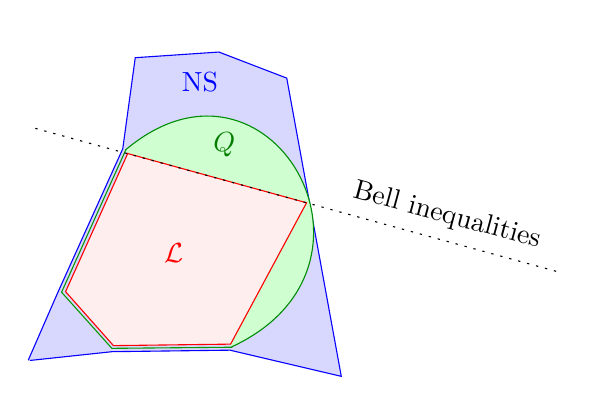
\begin{tikzpicture}[x=0.75pt,y=0.75pt,yscale=-1,xscale=1]
%uncomment if require: \path (0,300); %set diagram left start at 0, and has height of 300

%Straight Lines [id:da23136337283083197] 
\draw [color={rgb, 255:red, 7; green, 0; blue, 255 }  ,draw opacity=1 ][fill={rgb, 255:red, 216; green, 216; blue, 255 }  ,fill opacity=1 ]   (193.24,212.35) -- (232.84,208.12) -- (289.68,207.39) -- (343.3,220) -- (317.02,76.32) -- (284.32,63.75) -- (244.03,66.48) -- (238.01,110.36) -- (206.66,179.74) -- (192.47,212.25) ;


%Curve Lines [id:da7638922601289366] 
\draw [color={rgb, 255:red, 0; green, 141; blue, 5 }  ,draw opacity=1 ][fill={rgb, 255:red, 207; green, 255; blue, 209 }  ,fill opacity=1 ]   (290.45,205.8) .. controls (374.54,167.01) and (308.55,52.28) .. (239.22,111.01) ;


%Straight Lines [id:da5242020331974522] 
\draw [color={rgb, 255:red, 255; green, 0; blue, 0 }  ,draw opacity=1 ][fill={rgb, 255:red, 255; green, 238; blue, 238 }  ,fill opacity=1 ]   (240.53,112.33) -- (210.46,179.2) -- (233.52,205.2) -- (289.97,204.48) -- (326.56,136.37) -- (240.53,112.69) ;


%Straight Lines [id:da9957536132619464] 
\draw [color={rgb, 255:red, 10; green, 153; blue, 0 }  ,draw opacity=1 ]   (239.47,110.9) -- (208.53,179.47) -- (232.76,206.51) -- (290.86,205.97) ;


%Straight Lines [id:da34626836175073983] 
\draw  [dash pattern={on 0.84pt off 2.51pt}]  (195.89,100.52) -- (449.07,170.01) ;



% Text Node
\draw (262.5,160.59) node [color={rgb, 255:red, 255; green, 0; blue, 0 }  ,opacity=1 ]  {$\mathcal{L}$};
% Text Node
\draw (286.9,108.64) node [color={rgb, 255:red, 4; green, 124; blue, 0 }  ,opacity=1 ]  {$Q$};
% Text Node
\draw (275.22,78.23) node [color={rgb, 255:red, 0; green, 6; blue, 255 }  ,opacity=1 ]  {$\mathrm{NS}$};
% Text Node
\draw (394.18,142.69) node [rotate=-15.13] [align=left] {Bell inequalities};


\end{tikzpicture}
\caption{Schema delle relazioni tra i possibili insiemi di scenari di Bell, delimitati da vincoli nello spazio $\mathcal{P}$ (qui proiettati in $d=2$). Si trova infatti che $\op{NS}$ ha la struttura di un \textit{politopo}. I piani che separano le varie classi sono detti, in generale, \textbf{disuguaglianze di Bell}.\label{fig:classi-scenariBell}}
\end{figure}
\end{enumerate}

Nel caso $\Delta =2$, $m=2$, la forma più generale delle disuguaglianze di Bell è data da:
\begin{align*}
S \cdot p = \sum_{abXY} S_{XY}^{ab} p(ab|XY) \leq S_k
\end{align*}


\begin{figure}[H]
\centering
\tikzset{every picture/.style={line width=0.75pt}} %set default line width to 0.75pt        

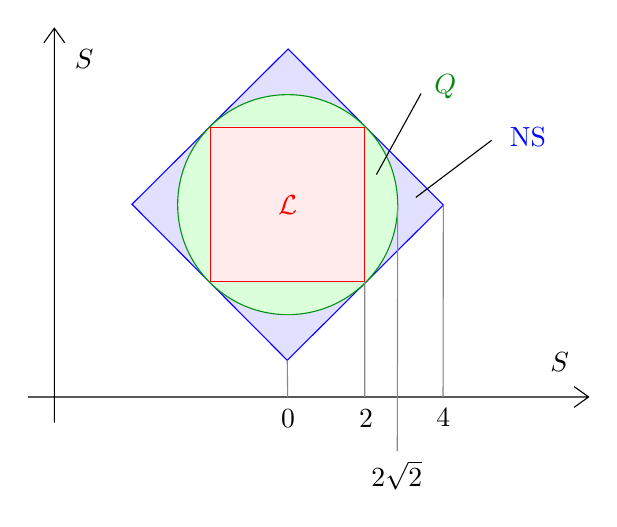
\begin{tikzpicture}[x=0.75pt,y=0.75pt,yscale=-1,xscale=1]
%uncomment if require: \path (0,300); %set diagram left start at 0, and has height of 300

%Shape: Rectangle [id:dp30928970522637145] 
\draw  [color={rgb, 255:red, 11; green, 0; blue, 255 }  ,draw opacity=1 ][fill={rgb, 255:red, 225; green, 225; blue, 255 }  ,fill opacity=1 ] (240,114.8) -- (315.2,40) -- (390,115.2) -- (314.8,190) -- cycle ;
%Shape: Ellipse [id:dp9930572540891616] 
\draw  [color={rgb, 255:red, 0; green, 148; blue, 16 }  ,draw opacity=1 ][fill={rgb, 255:red, 219; green, 255; blue, 219 }  ,fill opacity=1 ] (261.99,115) .. controls (261.99,85.72) and (285.72,61.99) .. (315,61.99) .. controls (344.28,61.99) and (368.01,85.72) .. (368.01,115) .. controls (368.01,144.28) and (344.28,168.01) .. (315,168.01) .. controls (285.72,168.01) and (261.99,144.28) .. (261.99,115) -- cycle ;
%Shape: Axis 2D [id:dp5751847689571885] 
\draw  (190,207.65) -- (460,207.65)(202.57,30) -- (202.57,220) (453,202.65) -- (460,207.65) -- (453,212.65) (197.57,37) -- (202.57,30) -- (207.57,37)  ;
%Shape: Rectangle [id:dp8277993508737616] 
\draw  [color={rgb, 255:red, 255; green, 0; blue, 0 }  ,draw opacity=1 ][fill={rgb, 255:red, 255; green, 235; blue, 235 }  ,fill opacity=1 ] (277.89,77.89) -- (352.11,77.89) -- (352.11,152.11) -- (277.89,152.11) -- cycle ;
%Straight Lines [id:da3288239217718776] 
\draw [color={rgb, 255:red, 136; green, 136; blue, 136 }  ,draw opacity=1 ][fill={rgb, 255:red, 0; green, 0; blue, 0 }  ,fill opacity=1 ]   (352.11,152.11) -- (352.14,207.57) ;


%Straight Lines [id:da5700506077210445] 
\draw [color={rgb, 255:red, 136; green, 136; blue, 136 }  ,draw opacity=1 ][fill={rgb, 255:red, 0; green, 0; blue, 0 }  ,fill opacity=1 ]   (368.01,115) -- (367.86,207.57) ;


%Straight Lines [id:da9368725092254024] 
\draw [color={rgb, 255:red, 136; green, 136; blue, 136 }  ,draw opacity=1 ][fill={rgb, 255:red, 0; green, 0; blue, 0 }  ,fill opacity=1 ]   (390,115.2) -- (389.85,207.77) ;


%Straight Lines [id:da9435052139977784] 
\draw [color={rgb, 255:red, 136; green, 136; blue, 136 }  ,draw opacity=1 ][fill={rgb, 255:red, 0; green, 0; blue, 0 }  ,fill opacity=1 ]   (367.86,207.57) -- (367.8,233.8) ;


%Straight Lines [id:da06475354051924254] 
\draw    (357.75,100.5) -- (379.25,61.5) ;


%Straight Lines [id:da9429638260774549] 
\draw    (376.75,111.5) -- (413.25,84) ;


%Straight Lines [id:da0310564865217966] 
\draw [color={rgb, 255:red, 136; green, 136; blue, 136 }  ,draw opacity=1 ][fill={rgb, 255:red, 0; green, 0; blue, 0 }  ,fill opacity=1 ]   (314.8,190) -- (315,207.8) ;



% Text Node
\draw (352.8,218.2) node   {$2$};
% Text Node
\draw (367.6,245.4) node   {$2\sqrt{2}$};
% Text Node
\draw (390,217.8) node   {$4$};
% Text Node
\draw (446,191) node   {$S$};
% Text Node
\draw (217,45) node   {$S$};
% Text Node
\draw (315,115) node [color={rgb, 255:red, 255; green, 0; blue, 0 }  ,opacity=1 ]  {$\mathcal{L}$};
% Text Node
\draw (390.9,58.14) node [color={rgb, 255:red, 1; green, 139; blue, 12 }  ,opacity=1 ]  {$Q$};
% Text Node
\draw (430.72,82.23) node [color={rgb, 255:red, 0; green, 6; blue, 255 }  ,opacity=1 ]  {$\mathrm{NS}$};
% Text Node
\draw (315.2,218.2) node   {$0$};


\end{tikzpicture}
\caption{Relazioni tra $Q$, $\mathcal{L}$ e $\op{NS}$ per $\Delta=2$, $m=2$.\label{fig:delta2-rel}}
\end{figure}

\begin{comment}
\section{Dense Coding e correlazioni classiche}
Abbiamo visto che inviando un qubit è possibile trasmettere $2$ bit classici in una volta sola.\\
Ci chiediamo: è possibile farlo anche partendo da stati correlati in senso classico?\\

Nel formalismo delle matrici densità, uno stato entangled è:
\begin{align*}
\ket{\psi} &= \frac{1}{\sqrt{2}}(\ket{00}+\ket{11}) \Rightarrow  \rho=\ket{\psi}\bra{\psi} = \frac{1}{2}(\ket{00}+\ket{11})(\bra{00}+\bra{11})=\\
 &= \frac{1}{2}(\ket{00}\bra{00} + \ket{00}\bra{11} + \ket{11}\bra{00} + \ket{11}\bra{11}) =\\
&= \frac{1}{2}\begin{pmatrix}1 & 0 & 0 & 1\\
0 & 0 & 0 & 0\\
0 & 0 & 0 & 0\\
1 & 0 & 0 & 1\end{pmatrix}
\end{align*}
D'altro canto, uno stato di correlazione classica è una mistura statistica:
\begin{align*}
\rho = \sum_k p_k \ket{\psi_k}\bra{\psi_k}
\end{align*}
Per esempio:
\begin{align*}
\rho = \frac{1}{2}\ket{00}\bra{00} + \frac{1}{2}\ket{11}\bra{11} = \frac{1}{2}\begin{pmatrix}1 & 0 & 0 & 0\\
0 & 0 & 0 & 0\\
0 & 0 & 0 & 0\\
0 & 0 & 0 & 1
\end{pmatrix}
\end{align*}
\end{comment}

\section{Misura sperimentale della violazione delle disuguaglianze CHSH}
Esaminiamo ora un possibile apparato sperimentale in grado di osservare la violazione delle disuguaglianze CHSH.\\
Utilizzeremo come qubit lo stato di polarizzazione di un fotone, nella base $\{\ket{H},\ket{V}\}$ di polarizzazione (lineare) orizzontale (H) o verticale (V).\\
Per generare qubit entangled impieghiamo il fenomeno di \textit{spontaneous parametric downconversion}. Certi cristalli (come ad esempio il borato di Bario, comunemente detto BBO) esibiscono un comportamento ottico \textbf{non lineare}. Ciò rende possibile la conversione di un fotone in ingresso in una coppia di fotoni, rispettando conservazione di energia e momento (figura \ref{fig:spdc}).

\begin{figure}[H]
    \centering
    \begin{subfigure}[t]{0.5\textwidth}
        \centering
        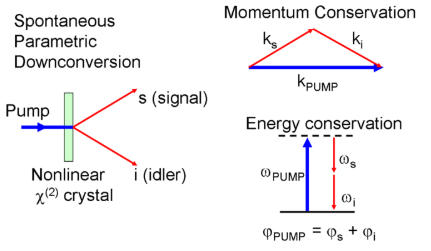
\includegraphics[width=0.8\textwidth]{Immagini/28_3/spdc_1.PNG}
    \end{subfigure}%
    \begin{subfigure}[t]{0.5\textwidth}
        \centering
        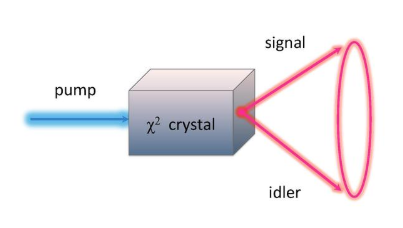
\includegraphics[width=0.8\textwidth]{Immagini/28_3/spdc_2.PNG}
    \end{subfigure}
    \caption{A sinistra: schema del processo di \textit{spontaneous parametric downconversion}. Come visibile a destra, i due fotoni risultanti sono emessi in un cono di angolo specifico.}
    \label{fig:spdc}
\end{figure}

Tale processo avviene con un'efficienza molto ridotta, e solo per certe frequenze dei fotoni in ingresso. Per poterlo sfruttare, perciò, è necessario utilizzare un laser sufficientemente potente.\\

A seconda della tipologia di cristallo, la polarizzazione dei due fotoni emessi è più o meno correlata a quella del fotone incidente. In particolare, in un cristallo con \textit{phase matching} di tipo $1$, se il fotone iniziale è polarizzato parallelamente ad uno specifico asse del cristallo, allora i due fotoni risultanti hanno entrambi la stessa polarizzazione, perpendicolare a quella iniziale.\\
Ciò permette, per esempio, di convertire un fotone $\ket{V}$ in due fotoni $\ket{H}$:
\begin{align*}
    \ket{V} \mapsto \ket{H}_A \otimes \ket{H}_B
\end{align*}
Lo stato così generato è separabile, e quindi non entangled. Possiamo rimediare a ciò sovrapponendo due cristalli non lineari, con assi perpendicolari, e illuminandoli con luce polarizzata a $45^\circ$ (figura \ref{fig:entanglement_gen}). Il fotone iniziale è quindi nello stato $\ket{\psi_1}$:
\begin{align*}
    \ket{\psi_1} = \frac{1}{\sqrt{2}}(\ket{H} + \ket{V})
\end{align*}
e perciò ha uguale probabilità di dividersi in due fotoni polarizzati orizzontalmente o verticalmente, a seconda del cristallo con cui interagisce.

\begin{figure}[H]
    \centering
    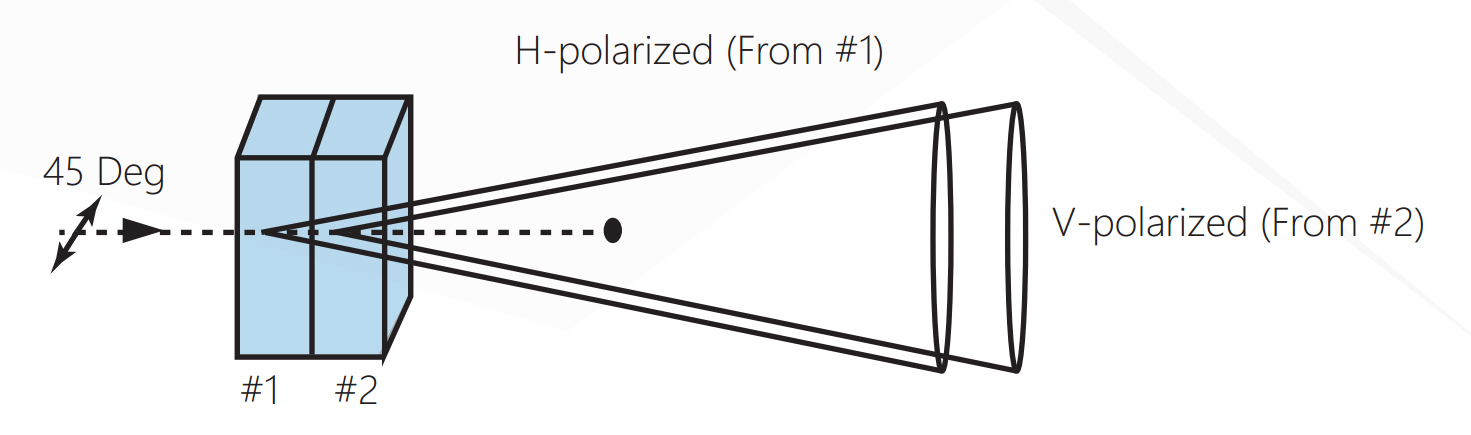
\includegraphics[width=0.7\textwidth]{Immagini/28_3/entanglement_gen.jpg}
    \caption{I cristalli $\#1$ e $\#2$ hanno assi ottici perpendicolari: il primo verticale, il secondo orizzontale. Perciò $\#1$ converte fotoni $\ket{V} \to \ket{H}\otimes \ket{H}$, mentre il secondo $\ket{H} \to \ket{V}\otimes \ket{V}$. Utilizzando come input fotoni polarizzati a $45^\circ$ (sovrapposizione a pari coefficienti di $\ket{H}$ e $\ket{V}$) allora ogni fotone ha pari probabilità di essere splittato da $\#1$ o da $\#2$. Fino a quando non viene fatta una misura, entrambi i processi \textit{sono esplorati}, e perciò lo stato finale è entangled.}
    \label{fig:entanglement_gen}
\end{figure}

L'unico problema è che, a causa dello spessore dei cristalli non lineari, i due \textit{coni} di emissione delle coppie di fotoni non coincidono. Perciò i due percorsi possibili (split nel primo cristallo o nel secondo) non sono perfettamente sovrapposti - e quindi lo stato finale non è una superposizione coerente, ma uno stato misto:
\begin{align*}
    \ket{\psi_2'} = \frac{1}{2}(\ket{HH}\bra{HH} + \ket{VV}\bra{VV})
\end{align*}
Tale fenomeno è definito \textit{walk-off}, e può essere compensato \q{ritardando} uno dei due fotoni tramite un altro elemento ottico. Così facendo otteniamo, finalmente, uno stato entangled coerente:
\begin{align*}
    \ket{\psi_2} = \frac{1}{\sqrt{2}}(\ket{H}_A \ket{H}_B + e^{i\varphi} \ket{V}_A \ket{V}_B)
\end{align*}

Non resta altro che effettuare misure di polarizzazione sui due fotoni entangled. Per farlo, esaminiamo - punto per punto - il seguente setup:
\begin{figure}[H]
    \centering
    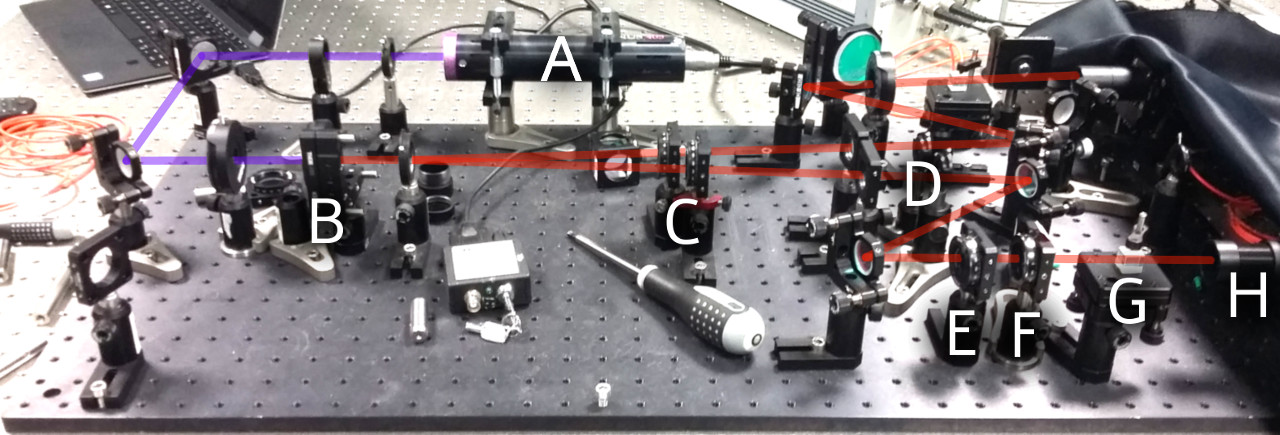
\includegraphics[width=\textwidth]{Immagini/28_3/Bell_setup.jpg}
    \caption{Setup sperimentale per la violazione delle disuguaglianze CHSH}
    \label{fig:bell-setup}
\end{figure}

\begin{enumerate}
    \item In \textbf{A} si ha un laser di un'opportuna lunghezza d'onda (specifica per i BBO) e sufficientemente potente. Il fascio viene polarizzato \textbf{verticalmente} da un filtro.
    \item Il laser viene focalizzato e collimato da alcuni elementi ottici, e tramite una coppia di specchi viene fatto incidere sul cristallo non lineare in \textbf{B}, dove avviene il fenomeno di \textit{parametric down-conversion}.
    \item Ci concentriamo su uno specifico piano all'interno del cono di emissione delle coppie di fotoni. In \textbf{C}, tramite opportuni elementi ottici, si sovrappongono i due coni relativi ai due strati di cristallo non lineare, in modo da ottenere lo stato coerente $\ket{\psi_2}$.
    \item Dopo aver attraversato un'ulteriore lente, in \textbf{D} i due fasci di fotoni entangled incidono su una coppia di \textit{iridi}, che vengono regolati in modo da lasciar passare solo la componente effettivamente sovrapposta (dove quindi l'entanglement è massimo)
    \item Ciascun fascio viene riflesso verso l'apparato di misura. Concentriamoci sul fascio inferiore. In \textbf{E} si ha una lamina $\lambda/2$, che consente di variare l'angolo $\theta$ di polarizzazione lineare della luce incidente. Nel dettaglio, la lamina \q{riflette} la polarizzazione della luce incidente rispetto al suo asse ottico (che può essere orientato a piacere):
    \begin{figure}[H]
        \centering
        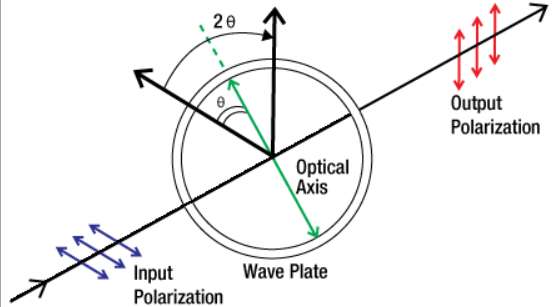
\includegraphics[width=0.6\textwidth]{Immagini/28_3/lambda2.PNG}
        \caption{Schema del funzionamento di una lamina $\lambda/2$. Poiché la lamina \q{riflette} la polarizzazione incidente, orientandola a $\theta = 45^\circ$ è possibile convertire $\ket{H}$ in $\ket{V}$ (e viceversa). Analogamente, per $\theta=22.5^\circ$, si converte una polarizzazione a $45^\circ$ ($\ket{+}$) in $\ket{H}$.}
        \label{fig:my_label}
    \end{figure}
    Una lamina $\lambda/4$ (in \textbf{F}) è presente in uno solo dei due fasi, e serve a fissare la fase $\varphi$ che compare in $\ket{\psi_2}$. A questo punto il fascio incide su un \q{polarizing biscuit} in \textbf{G}, che è un normale cristallo birifrangente orientato in modo da trasmettere al $100\%$ la componente $\ket{H}$, e da riflettere quella $\ket{V}$. Poiché possiamo convertire una qualsiasi polarizzazione in $\ket{H}$ orientando opportunamente la lamina $\lambda/2$, l'apparato consente di misurare la polarizzazione lungo un asse arbitrario.
    \item Infine, in \textbf{H}, si ha un rivelatore a singolo fotone, collegato ad un'opportuna elettronica di acquisizione e ad un computer per la presa dati.
\end{enumerate}

Per determinare la presenza o meno di entanglement, un modo è misurare un'osservabile detta \textbf{entanglement witness}, tale da risultare in esiti differenti per stati separabili o stati entangled.\\
Un esempio è misurare le correlazioni in \textit{basi coniugate}. Ci aspettiamo infatti di osservare coppie polarizzate $HH$ o $VV$ sia per $\ket{\psi_2}$ che per $\ket{\psi_2'}$, e allo stesso modo di non osservare $HV$ e $VH$ (se non per le incertezze sperimentali dovute ad allineamento, rumore, etc.). Tuttavia, misurando in una base \textit{diagonale}, per $\ket{\psi_2}$ ci aspettiamo di misurare tanti fotoni polarizzati $++$, e nessuno $+-$, mentre per $\ket{\psi_2'}$ misureremo fotoni con ogni combinazione di polarizzazione ($++$ e $+-$ allo stesso modo).\\

In presenza di entanglement possiamo misurare la violazione delle disuguaglianze di Bell. L'idea è di misurare un fotone nelle polarizzazioni orizzontale e verticale, e l'altro in diagonale e antidiagonale, eseguendo quanto già visto in (\ref{eqn:S-Bell}). 

\end{document}

